\documentclass[tikz,border=10pt]{standalone}
\usepackage{tikz}
\usetikzlibrary{shapes, arrows, positioning, fit, shadows, backgrounds, calc}

\begin{document}

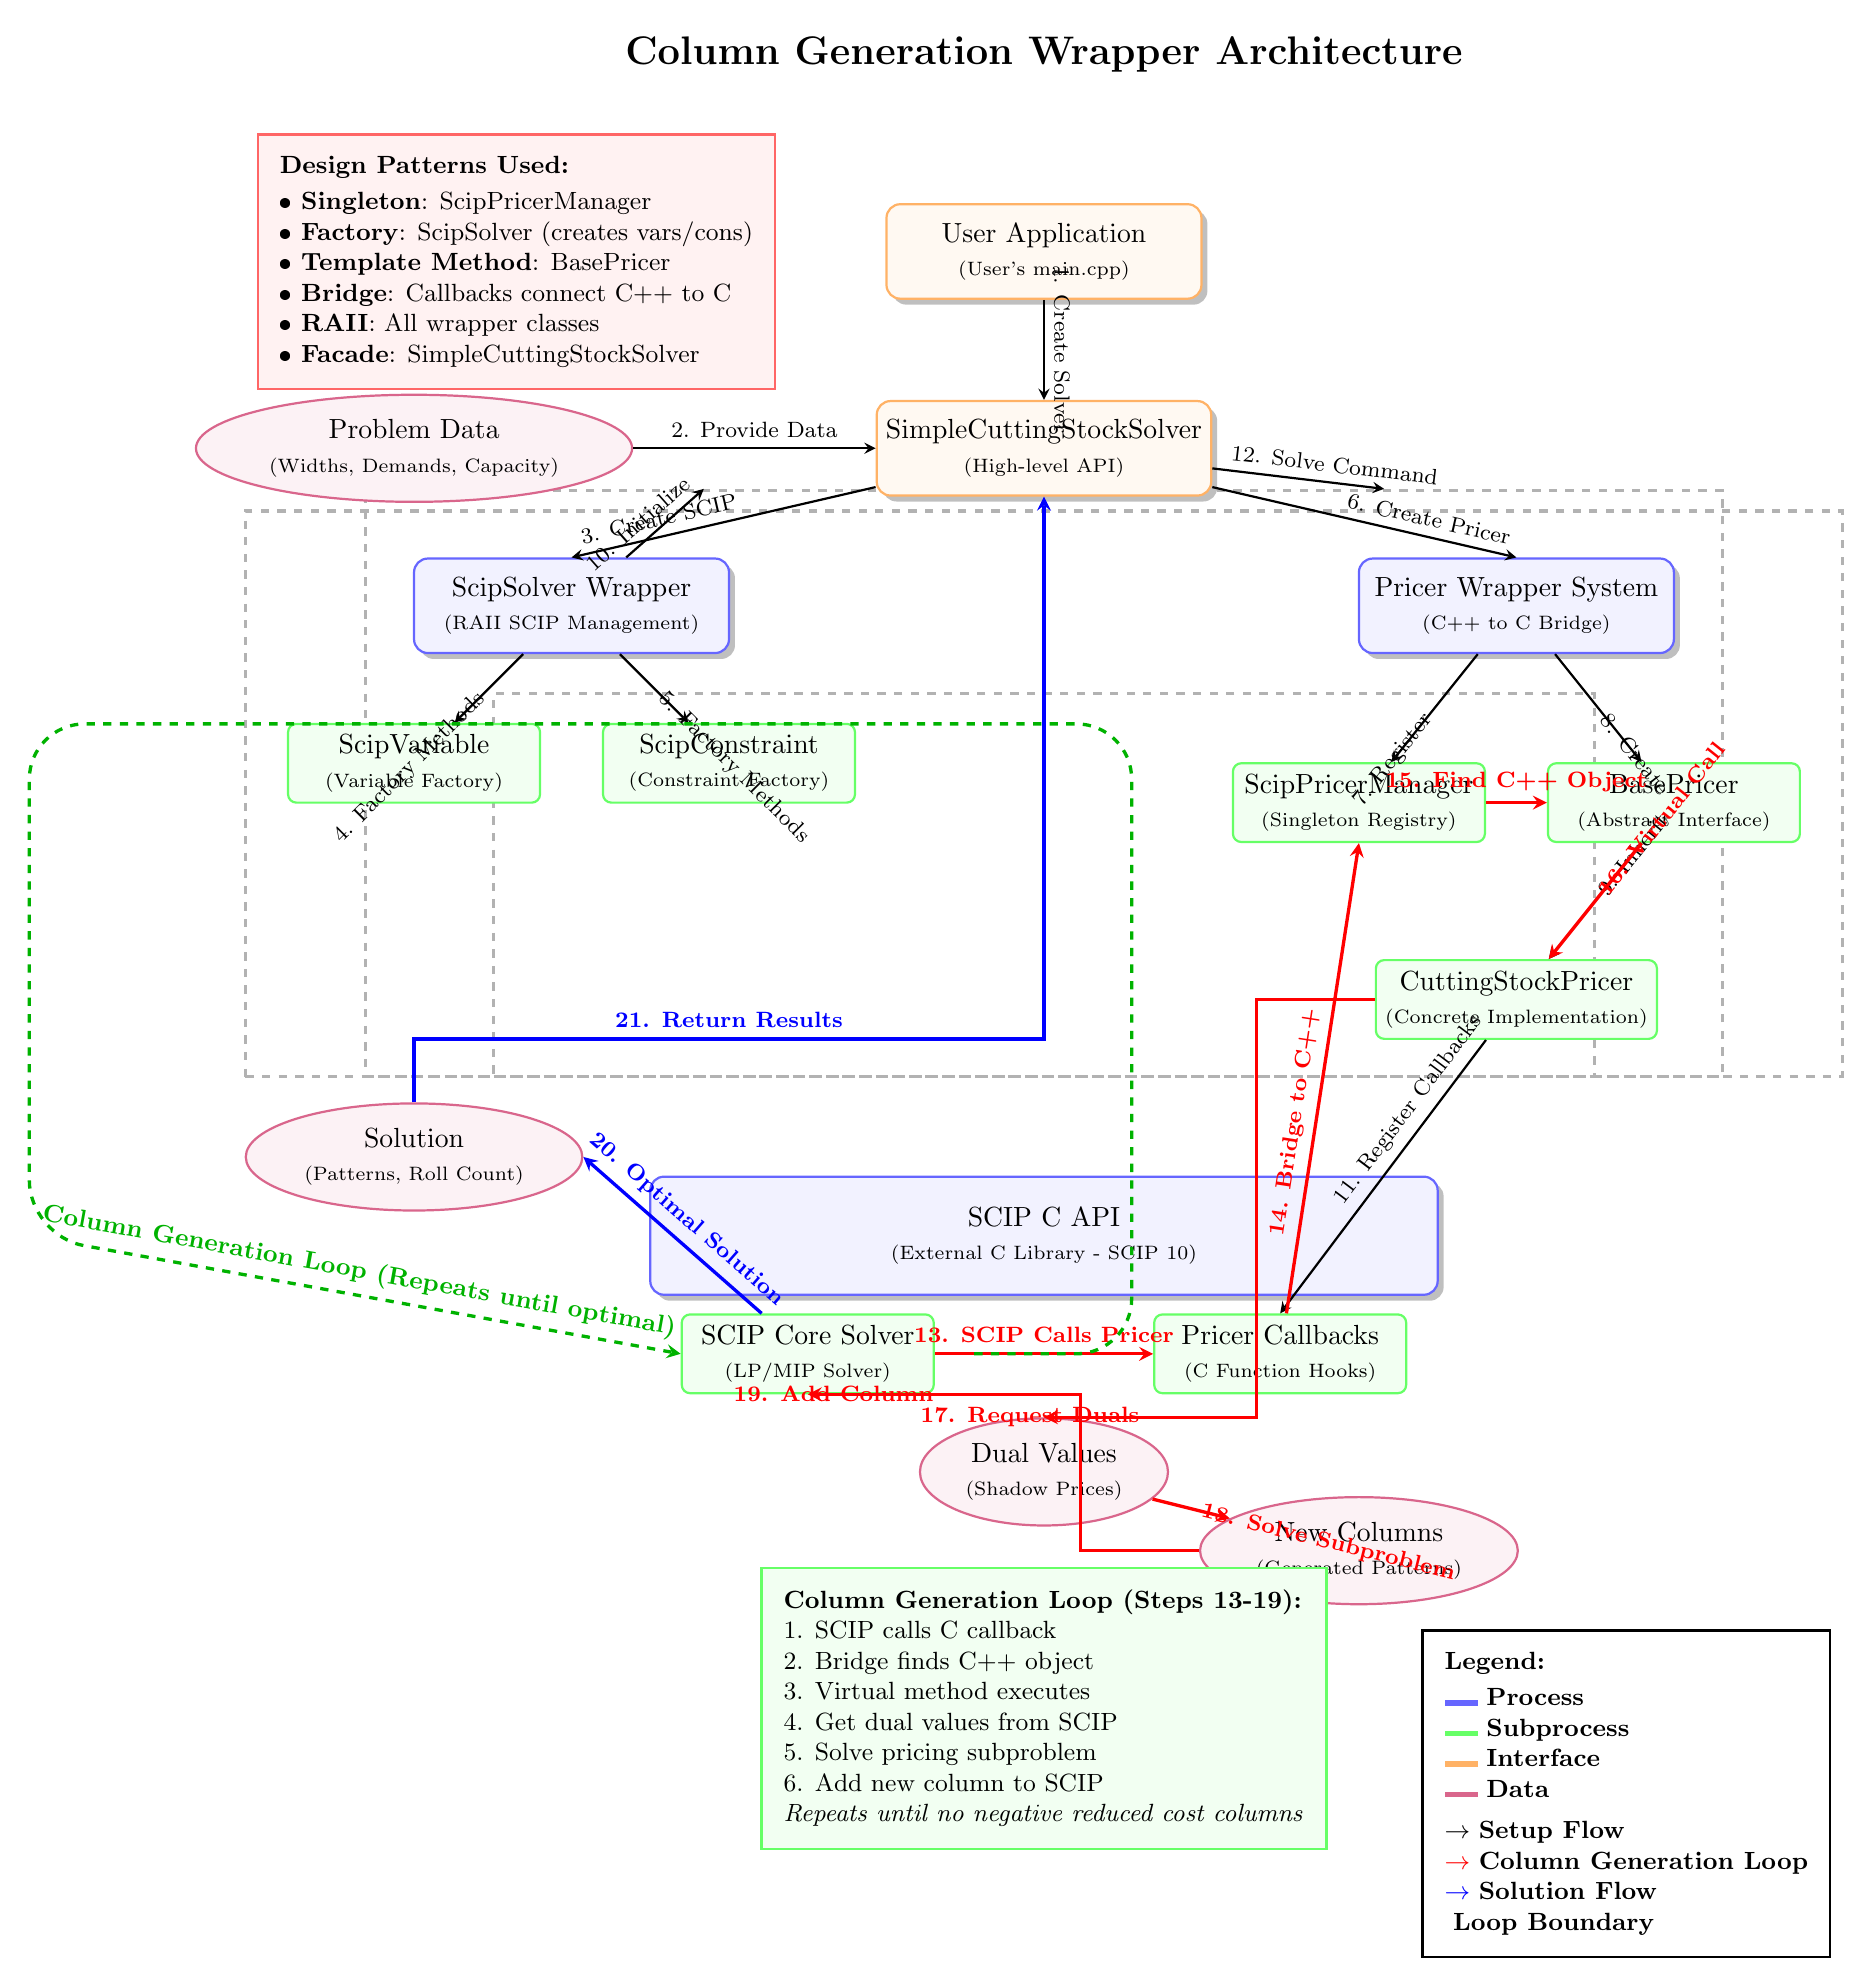
\begin{tikzpicture}[
    % Define styles
    process/.style={rectangle, draw=blue!60, fill=blue!5, thick, minimum height=1.2cm, minimum width=4cm, align=center, rounded corners=5pt, drop shadow},
    subprocess/.style={rectangle, draw=green!60, fill=green!5, thick, minimum height=1cm, minimum width=3.2cm, align=center, rounded corners=3pt},
    interface/.style={rectangle, draw=orange!60, fill=orange!5, thick, minimum height=1.2cm, minimum width=4cm, align=center, rounded corners=5pt, drop shadow},
    data/.style={ellipse, draw=purple!60, fill=purple!5, thick, minimum height=1cm, minimum width=2.5cm, align=center},
    arrow/.style={->, >=stealth, thick},
    dashedarrow/.style={->, >=stealth, thick, dashed},
    label/.style={midway, above, sloped, font=\footnotesize},
    container/.style={rectangle, draw=gray!60, dashed, very thick, inner sep=15pt},
    title/.style={font=\Large\bfseries, align=center}
]

% Title
\node[title] at (0, 13) {Column Generation Wrapper Architecture};

% ============================================================================
% USER LAYER (Simplified Interface)
% ============================================================================
\node[interface] (user) at (0, 10.5) {User Application\\\scriptsize(User's main.cpp)};
\node[interface] (simplesolver) at (0, 8) {SimpleCuttingStockSolver\\\scriptsize(High-level API)};

% ============================================================================
% WRAPPER LAYER - LEFT SIDE (SCIP Wrapper)
% ============================================================================
\node[process] (scipsolver) at (-6, 6) {ScipSolver Wrapper\\\scriptsize(RAII SCIP Management)};
\node[subprocess] (scipvar) at (-8, 4) {ScipVariable\\\scriptsize(Variable Factory)};
\node[subprocess] (scipcons) at (-4, 4) {ScipConstraint\\\scriptsize(Constraint Factory)};

% ============================================================================
% WRAPPER LAYER - RIGHT SIDE (Pricer System)
% ============================================================================
\node[process] (pricerwrapper) at (6, 6) {Pricer Wrapper System\\\scriptsize(C++ to C Bridge)};
\node[subprocess] (manager) at (4, 3.5) {ScipPricerManager\\\scriptsize(Singleton Registry)};
\node[subprocess] (basepricer) at (8, 3.5) {BasePricer\\\scriptsize(Abstract Interface)};
\node[subprocess] (stockpricer) at (6, 1) {CuttingStockPricer\\\scriptsize(Concrete Implementation)};

% ============================================================================
% SCIP LAYER (C API Integration)
% ============================================================================
\node[process, minimum width=10cm, minimum height=1.5cm] (scipapi) at (0, -2) {SCIP C API\\\scriptsize(External C Library - SCIP 10)};
\node[subprocess] (scipcore) at (-3, -3.5) {SCIP Core Solver\\\scriptsize(LP/MIP Solver)};
\node[subprocess] (pricercallbacks) at (3, -3.5) {Pricer Callbacks\\\scriptsize(C Function Hooks)};

% ============================================================================
% DATA FLOW ELEMENTS
% ============================================================================
\node[data] (problemdata) at (-8, 8) {Problem Data\\\scriptsize(Widths, Demands, Capacity)};
\node[data] (solution) at (-8, -1) {Solution\\\scriptsize(Patterns, Roll Count)};
\node[data] (dualvalues) at (0, -5) {Dual Values\\\scriptsize(Shadow Prices)};
\node[data] (newcolumns) at (4, -6) {New Columns\\\scriptsize(Generated Patterns)};

% ============================================================================
% CONTAINERS (Architecture Layers)
% ============================================================================
\begin{scope}[on background layer]
    \node[container, fit=(user) (simplesolver) (problemdata), label={[anchor=north]90:\textbf{USER LAYER}}] (userlayer) {};
    \node[container, fit=(scipsolver) (scipvar) (scipcons) (pricerwrapper) (manager) (basepricer) (stockpricer), 
          label={[anchor=north]90:\textbf{WRAPPER LAYER (C++ Classes)}}] (wrapperlayer) {};
    \node[container, fit=(scipapi) (scipcore) (pricercallbacks) (dualvalues) (newcolumns) (solution), 
          label={[anchor=north]90:\textbf{SCIP LAYER (C API Integration)}}] (scipapi) {};
\end{scope}

% ============================================================================
% SETUP PHASE ARROWS
% ============================================================================

% User creates solver
\draw[arrow] (user) -- node[label] {1. Create Solver} (simplesolver);

% Solver receives problem data
\draw[arrow] (problemdata) -- node[label] {2. Provide Data} (simplesolver);

% Solver creates SCIP wrapper
\draw[arrow] (simplesolver) -- node[label, pos=0.7] {3. Create SCIP} (scipsolver.north);

% SCIP wrapper creates factories
\draw[arrow] (scipsolver) -- node[label, left] {4. Factory Methods} (scipvar);
\draw[arrow] (scipsolver) -- node[label, right] {5. Factory Methods} (scipcons);

% Solver creates pricer system
\draw[arrow] (simplesolver) -- node[label, pos=0.7] {6. Create Pricer} (pricerwrapper.north);

% Pricer system setup
\draw[arrow] (pricerwrapper) -- node[label, left] {7. Register} (manager);
\draw[arrow] (pricerwrapper) -- node[label, right] {8. Create} (basepricer);
\draw[arrow] (basepricer) -- node[label, right] {9. Inherit} (stockpricer);

% ============================================================================
% INTEGRATION WITH SCIP
% ============================================================================

% SCIP wrapper initializes SCIP
\draw[arrow] (scipsolver) -- node[label, pos=0.3] {10. Initialize} 
    ($(scipapi.north west)!0.25!(scipapi.north east)$);

% Pricer registers callbacks with SCIP
\draw[arrow] (stockpricer) -- node[label, pos=0.3] {11. Register Callbacks} 
    (pricercallbacks.north);

% ============================================================================
% SOLVING PHASE - COLUMN GENERATION LOOP
% ============================================================================

% Start solving
\draw[arrow] (simplesolver) -- node[label, pos=0.7] {12. Solve Command} 
    ($(scipapi.north west)!0.75!(scipapi.north east)$);

% SCIP calls pricer (Loop Step 1)
\draw[arrow, red, very thick] (scipcore) -- node[label, above] {\textbf{13. SCIP Calls Pricer}} 
    (pricercallbacks);

% Bridge to C++ (Loop Step 2)
\draw[arrow, red, very thick] (pricercallbacks) -- 
    node[label, above, pos=0.4] {\textbf{14. Bridge to C++}} 
    (manager.south);

% Virtual dispatch (Loop Step 3)
\draw[arrow, red, very thick] (manager) -- 
    node[label, above] {\textbf{15. Find C++ Object}} (basepricer);
    
\draw[arrow, red, very thick] (basepricer) -- 
    node[label, right] {\textbf{16. Virtual Call}} (stockpricer);

% Get dual values (Loop Step 4)
\draw[arrow, red, very thick] (stockpricer.west) -- ++(-1.5,0) |-
    node[label, pos=0.75, left] {\textbf{17. Request Duals}} 
    (dualvalues.north);

% Solve knapsack (Loop Step 5)
\draw[arrow, red, very thick] (dualvalues) -- 
    node[label, right] {\textbf{18. Solve Subproblem}} (newcolumns);

% Add column to SCIP (Loop Step 6)
\draw[arrow, red, very thick] (newcolumns.west) -- ++(-1.5,0) |-
    node[label, pos=0.75, left] {\textbf{19. Add Column}} 
    (scipcore.south);

% ============================================================================
% SOLUTION RETRIEVAL
% ============================================================================

% SCIP returns solution
\draw[arrow, blue, very thick] (scipcore) -- 
    node[label, above] {\textbf{20. Optimal Solution}} 
    (solution.east);

% Solver displays results
\draw[arrow, blue, very thick] (solution) -- ++(0,1.5) -|
    node[label, pos=0.25, above] {\textbf{21. Return Results}} 
    (simplesolver.south);

% ============================================================================
% LOOP BACK ARROW (Shows iteration)
% ============================================================================
\draw[arrow, dashed, green!70!black, very thick, rounded corners=20pt] 
    ($(scipcore.east)+(0.5,0)$) -- ++(2,0) -- ++(0,8) -- ++(-14,0) -- 
    ++(0,-6.5) -- (scipcore.west)
    node[midway, above, sloped, font=\small\bfseries, green!70!black] 
    {Column Generation Loop (Repeats until optimal)};

% ============================================================================
% LEGEND (Bottom Right)
% ============================================================================
\node[draw=black, thick, inner sep=8pt, align=left, font=\small, anchor=north east] 
    at (10, -7) {
    \textbf{Legend:}\\[2pt]
    \textcolor{blue!60}{\rule{12pt}{2pt}} \textbf{Process}\\
    \textcolor{green!60}{\rule{12pt}{2pt}} \textbf{Subprocess}\\
    \textcolor{orange!60}{\rule{12pt}{2pt}} \textbf{Interface}\\
    \textcolor{purple!60}{\rule{12pt}{2pt}} \textbf{Data}\\[4pt]
    \textcolor{black}{$\rightarrow$} \textbf{Setup Flow}\\
    \textcolor{red}{$\rightarrow$} \textbf{Column Generation Loop}\\
    \textcolor{blue}{$\rightarrow$} \textbf{Solution Flow}\\
    \textcolor{green!70!black}{$\circlearrowright$} \textbf{Loop Boundary}
};

% ============================================================================
% DESIGN PATTERNS BOX (Top Right)
% ============================================================================
\node[draw=red!60, thick, fill=red!5, inner sep=8pt, align=left, font=\small, anchor=north west] 
    at (-10, 12) {
    \textbf{Design Patterns Used:}\\[2pt]
    • \textbf{Singleton}: ScipPricerManager\\
    • \textbf{Factory}: ScipSolver (creates vars/cons)\\
    • \textbf{Template Method}: BasePricer\\
    • \textbf{Bridge}: Callbacks connect C++ to C\\
    • \textbf{RAII}: All wrapper classes\\
    • \textbf{Facade}: SimpleCuttingStockSolver
};

% ============================================================================
% KEY COMPONENTS BOX (Left Side)
% ============================================================================
% \node[draw=blue!60, thick, fill=blue!5, inner sep=8pt, align=left, font=\small, anchor=north west] 
%     at (-10, 6) {
%     \textbf{Key Components:}\\[2pt]
%     • \textbf{User Layer}: Clean API\\
%     • \textbf{Wrapper Layer}: C++ classes\\
%     • \textbf{SCIP Layer}: C API integration\\
%     • \textbf{Column Gen Loop}: Steps 13-19\\
%     • \textbf{Data Flow}: Arrows show movement\\
%     • \textbf{Control Flow}: Numbered steps
% };

% ============================================================================
% COLUMN GENERATION LOOP EXPLANATION
% ============================================================================
\node[draw=green!60, thick, fill=green!5, inner sep=8pt, align=left, font=\small] 
    at (0, -8) {
    \textbf{Column Generation Loop (Steps 13-19):}\\
    1. SCIP calls C callback\\
    2. Bridge finds C++ object\\
    3. Virtual method executes\\
    4. Get dual values from SCIP\\
    5. Solve pricing subproblem\\
    6. Add new column to SCIP\\
    \textit{Repeats until no negative reduced cost columns}
};

\end{tikzpicture}

\end{document}